\documentclass{article}

\usepackage[margin=1in]{geometry}
\usepackage{amsmath,amsthm,amssymb}
\usepackage{enumitem,epsfig}
\usepackage{graphicx}
\usepackage{rotating}
\usepackage{multirow}
\usepackage{float}
\usepackage{xcolor}
\usepackage{hyperref}
\usepackage{tikz}
\usetikzlibrary{shapes,arrows}

\def\x{\mathbf{x}}
\def\y{\mathbf{y}}
\def\v{\mathbf{v}}
\def\a{\mathbf{a}}
\def\b{\mathbf{b}}
\def\ttheta{(1-\theta)}
\def\A{\mathbf{A}}
\def\F{\mathbf{F}}
\def\I{\mathbf{I}}
\def\R{\mathbb{R}}
\def\C{\mathcal{C}}
\def\L{\mathcal{L}}

\title{Spring 2022 Term Project: Speaker Recognition\\ ECE 466 Digital Signal Processing}
\date{\today}
\author{}
\begin{document}

\maketitle

\section{Introduction}
Speaker recognition (not speech recognition), is a key area of research based on human voice signals. Given a set of individuals and their corresponding audio recordings, the aim is to identify the speaker in the audio signal automatically after tuning (or training) a digital system for the process. This process allows computers to verify the identity of speakers and control access to personalized, or even, secure information such as; banking by phone, remote access to computers, database access services, home speakers, shopping with home speakers, etc. This task is achieved by learning and utilizing speaker-specific characteristics of input utterances, and inspired heavily from human ears, and how they perceive sounds.

In this project, you will:
\begin{enumerate}
    \item Build a simple system for speaker recognition,
    \item Implement a procedure to preprocess data such that the data is safe, clean and reliable,
    \item Implement necessary machine learning building blocks, such as training, validation, testing
    \item Utilize multiple models/methods for preprocessing and classification, and compare them.
\end{enumerate}

\section{Principals of Speaker Recognition}
For a speaker recognition system, we might have two major tasks; identification and verification. Identification is the process of determining which registered speaker provides a given utterance. Verification, on the other hand, is the process of accepting or rejecting the identity claim of a speaker. The system that we will focus on is text-independent speaker identification system since its task is to identify the person who speaks regardless of what they are saying. This is akin to training and testing phases of a supervised machine learning system.

A speaker recognition system is built upon two modules: feature extraction and feature matching. Feature extraction is the process that extracts a small amount of data from the voice signal that can later be used to represent each speaker. This module is usually further tailored for other tasks as well, such as tailoring the features to help the feature matching, clean out data, anonymize the individuals, etc. Feature matching is the procedure to identify the unknown speaker by comparing extracted features from his/her voice input with the ones from a set of known speakers. 

Most speaker recognition systems are supervised, or semi-supervised. Therefore, they have a training and a testing phase. In the training phase, each registered speaker has to provide samples of their speech so that the system can build or train a reference model for that speaker. In the testing phase, the input speech is matched with stored reference model(s) and a recognition decision is made.

\section{Feature Extraction:}
This module will process the speech waveform for further analysis. The speech signal is a slowly time-varying signal but when examined over a sufficiently short period of time (between 5-100 ms), it's characteristics are often fairly stationary. However, over long periods of time (on the order of 1/5 seconds or more) the signal characteristic change to reflect the different speech sounds being spoken. Therefore, short-time Fourier analysis is the most common way to characterize the speech signal.

Different methods have been proposed to extract features from speech signals including Linear Prediction Coding (LPC), Mel-Frequency Cepstrum Coefficients (MFCC), and others.  MFCC is perhaps the best known and most popular and will be the focus of this project. MFCC's are based on the known variation of the human ear's critical bandwidths with frequency, filters spaced linearly at low frequencies and logarithmically at high frequencies have been used to capture the phonetically important characteristics of speech.  This is expressed in the mel-frequency scale, which is a linear frequency spacing below 1000 Hz and a logarithmic spacing above 1000 Hz.  The process of computing MFCCs is described in more detail next. In addition to MFCC's, we will also use simple FFT and STFT as naive ways of extracting features and see if these approaches are viable.

\subsection{Fast Fourier Transform Processor}
A simple idea is extracting frequency magnitudes as features of the signal. Since we are only interested in certain frequencies, the size of the features for each recording will be fixed. Fast Fourier Transform converts the speech signal from the time domain into the frequency domain.  The FFT is a fast algorithm to implement the Discrete Fourier Transform (DFT), which is defined on the set of values of speech signal $\{x_n\}$, as follows (see \href{https://docs.scipy.org/doc/scipy/reference/generated/scipy.fft.fft.html#scipy.fft.fft}{\texttt{scipy.fft.fft}}):
\begin{equation}
    X_k = \sum_{n=0}^{N-1} x_n e^{-j2\pi k n/N}, \qquad k\in\{1,2,\dots, N-1\}
\end{equation}
In general, $X_k$'s are complex numbers and we only consider their absolute values, i.e. magnitude part of FFT. The resulting sequence $\{X_k\}$ is interpreted as follows, positive frequencies $0\leq f < \frac{F_s}{2}$ correspond to values $0\leq n \leq \frac{N}{2}-1$, while negative frequencies $-\frac{F_s}{2}< f < 0$ correspond to $\frac{N}{2} \leq n \leq N-1$.  Here, $F_s$ denotes the sampling frequency. As we are not interested in frequencies above 5kHz, we will discard the corresponding elements of the resulting vector.

\subsection{Short Time Fourier Transform}
As speech signals are generally very long vectors, and frequency information changes throughout time, a better way of representing the frequency information is by separating the signal into smaller parts in time. This separation is can be achieved with overlapping frames. The frames of the signal, are then converted into frequency domain to get frequency information for each part. Thus, the whole process is akin to a moving FFT of the signal and the output has time and frequency information together. This way of processing a signal is usually called Short Time Fourier Transform (STFT) and the result is called a periodogram. A block diagram for STFT is given in Fig. \ref{fig:stft}.

\subsubsection{Frame Blocking}
In this step, the continuous speech signal is blocked into frames of N  samples, with adjacent frames being separated by $M (M < N)$.  The first frame consists of the first $N$ samples.  The second frame begins M samples after the first frame, and overlaps it by $N - M$ samples and so on.  This process continues until all the speech is accounted for within one or more frames.  Typical values for $N$ and $M$ are $N = 256$ (which is equivalent to ~ 30 msec windowing and facilitate the fast radix-2 FFT) and $M = 100$.

\subsubsection{Windowing}
The next step in the processing is to window each individual frame so as to minimize the signal discontinuities at the beginning and end of each frame. This is not a core part of STFT but it improves the results significantly. The concept here is to minimize the spectral distortion by using the window to taper the signal to zero at the beginning and end of each frame.  If we define the window as $w[n], 0\leq n\leq N-1$ , where $N$ is the number of samples in each frame, then the result of windowing is the signal:
\begin{equation}
    y_l[n] =x_l[n]w[n], \qquad 0\leq n \leq N.
\end{equation}
For this purpose, typically the Hamming window is used, which has the form (see \href{https://docs.scipy.org/doc/scipy-0.19.1/reference/generated/scipy.signal.hamming.html}{\texttt{scipy.signal.hamming}}):
\begin{equation}
    w(n) = 0.54 - 0.46 \cos\left(\frac{2\pi n}{N-1}\right)
\end{equation}

\subsubsection{Fast Fourier Transform}
The next processing step is converting each frame of $N$ samples from the time domain into the frequency domain using FFT. This creates a frequency/feature vector of length $N$ for each frame. We again consider only the magnitude part of FFT. Since we only consider the magnitude part, the output is the square root of the spectrogram of our signal. ({\it See the relationship between STFT and spectrogram \href{https://stackoverflow.com/questions/55683936/what-is-the-difference-between-scipy-signal-spectrogram-and-scipy-signal-stft}{in this StackOverflow question}.})

\subsection{Mel-frequency cepstrum coefficients processor}
A block diagram of the structure of an MFCC processor is given in Fig. \ref{fig:mfcc}. The speech input is typically recorded at a sampling rate above 10 kHz.  This sampling frequency was chosen to minimize the effects of aliasing in the analog-to-digital conversion.  These sampled signals can capture all frequencies up to 5 kHz, which cover most energy of sounds that are generated by humans.  As been discussed previously, the main purpose of the MFCC processor is to mimic the behavior of the human ears.  In addition, rather than the speech waveforms themselves, MFFC's are shown to be less susceptible to mentioned variations.

\def\pleft{120}
\def\pright{60}
\def\pmiddle{90}
\tikzstyle{block} = [rectangle, draw, fill=white!80!cyan,
    text width=5em, text centered, rounded corners, minimum height=4em]
\tikzstyle{block2} = [rectangle, draw, fill=white!80!green,
    text width=5em, text centered, rounded corners, minimum height=4em]
\tikzstyle{block3} = [rectangle, draw, fill=white!80!red,
    text width=5em, text centered, rounded corners, minimum height=4em]
\tikzstyle{line} = [draw, very thick, color=black!50, -latex']
\tikzset{
      left connect/.style = {line width=1pt, draw=blue!50!cyan!45!gray, -latex'},
      right connect/.style = {line width=1pt, draw=red!40!gray!60!orange, -latex'},
      middle connect/.style = {line width=1pt, draw=green!50!black!40!yellow, -latex'}
    }
\begin{figure}[htb]
    \centering
    \begin{tikzpicture}[scale=1, node distance = 3cm, auto]
        \path node (signal) {};
        \node [block, right of = signal, node distance=2.5cm] (frame) {Frame Blocking};
        \node [block, right of = frame] (windowing) {Windowing};
        \node [block, right of = windowing] (fft) {FFT};
        \node [right of = fft, node distance=2.8cm]  (stft) {};

        \path [right connect] (signal) -- node [above, color=black] {Speech} node [below,color=black] {Signal} (frame) ;
        \path [line] (frame) -- (windowing);
        \path [line] (windowing) -- (fft);
        \path [middle connect] (fft) --  node [above, color=black] {STFT} (stft); 
    \end{tikzpicture}
    \caption{Block Diagram of Short Time Fourier Transform.}
    \label{fig:stft}
\end{figure}
\begin{figure}[htb]
    \centering
    \begin{tikzpicture}[scale=1, node distance = 3cm, auto]
        \path node (speech) {};
        \node [block, right of = speech, node distance=2.5cm] (stft) {STFT};
        \node [block, right of = stft] (mfw) {Mel-frequency mapping};
        \node [block, right of = mfw] (dct) {DCT};
        \node [right of = dct, node distance=2.8cm]  (cepstrum) {};

        \path [right connect] (speech) -- node [above, color=black] {Speech} node [below,color=black] {Signal} (stft) ;
        \path [line] (stft) -- (mfw);
        \path [line] (mfw) -- (dct);
        \path [middle connect] (dct) --  node [above, color=black] {Cepstrum} (cepstrum); 
    \end{tikzpicture}
    \caption{Block Diagram of Mel-frequency pre-processing.}
    \label{fig:mfcc}
\end{figure}

\subsubsection{Mel-frequency Wrapping}
As mentioned above, psychophysical studies have shown that human perception of the frequency contents of sounds for speech signals does not follow a linear scale. Thus for each tone with an actual frequency, $f$, measured in Hz, a subjective pitch is measured on a scale called the 'mel' scale.  The mel-frequency scale is a linear frequency spacing below 1000 Hz and a logarithmic spacing above 1000 Hz.  

\begin{figure}[htb]
    \centering
    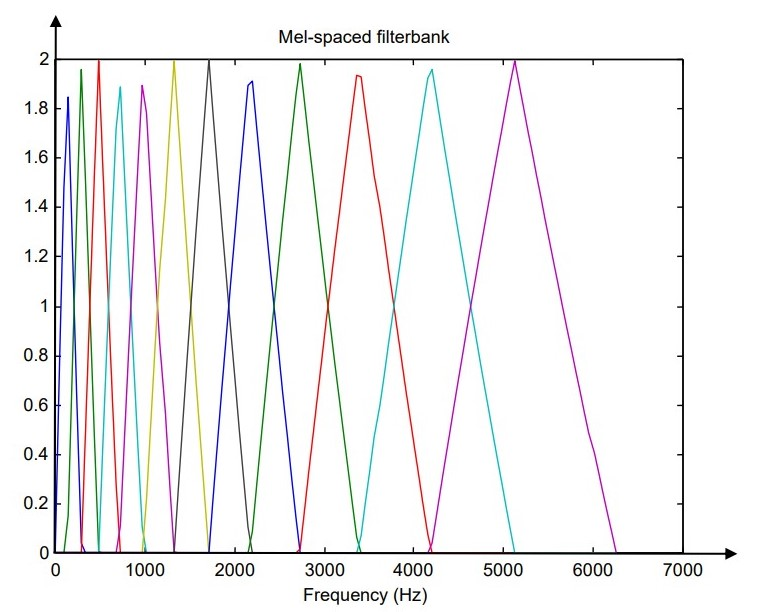
\includegraphics[width=.8\textwidth]{Fig2.jpg}
    \caption{An example of mel-spaced filterbank.}
\end{figure}

One approach to simulating the subjective spectrum is to use a filter bank, spaced uniformly on the mel-scale.  That filter bank has a triangular bandpass frequency response, and the spacing as well as the bandwidth is determined by a constant mel frequency interval.  The number of mel spectrum coefficients, $K$, is typically chosen as 20.  Note that this filter bank is applied in the frequency domain, thus it simply amounts to applying the triangle-shape windows as shown in the figure above to the spectrum, to the STFT of the signal.  A useful way of thinking about this mel-wrapping filter bank is to view each filter as a histogram bin (where bins have overlap) in the frequency domain. See \href{https://pytorch.org/audio/main/tutorials/audio_feature_extractions_tutorial.html#mel-filter-bank}{\texttt{melfilter}} function on Pytorch\footnote{You can also use the melfilter provided by \texttt{librosa} library or create your own function based on the source codes of these libraries.}. This function will create the triangular shape filters in the frequency domain. 
You need to filter each frame with each one of these filters to obtain the mel frequency cepstrum coefficients (MFCC) as discussed below.

\subsubsection{Cepstrum}
In this final step, we convert the log mel spectrum back to time.  The result is called the mel frequency cepstrum coefficients (MFCC).  The cepstral representation of the speech spectrum provides a good representation of the local spectral properties of the signal for the given frame analysis. Because the mel spectrum coefficients (and so their logarithm) are real numbers, we can convert them to the time domain using the Discrete Cosine Transform (DCT).  Therefore if we denote those mel power spectrum coefficients that are the result of the last step as $\tilde{S}_k$, $k\in\{1,2,\dots,K-1\}$, where $K$ is the number of filters, we can calculate the MFCC's, $\tilde{c}_n$, as: 
\begin{equation}
    \tilde{c}_n = \sum_{k=1}^K \log(\tilde{S}_k)\cos\left(n \left(k-\frac{1}{2}\right)\frac{\pi}{K}\right), \qquad n\in\{1,2,\dots,K-1\}.
\end{equation}
Note that we exclude the first component, $\tilde{c}_0$, from the DCT since it represents the mean value of the input signal, which carries little speaker specific information.

By applying the procedure described above, for each speech frame of around 30 ms with overlap, a set of mel-frequency cepstrum coefficients is computed.  These are the results of a cosine transform of the logarithm of the short-term power spectrum expressed on a mel-frequency scale.  This set of coefficients is called an acoustic vector.  Therefore each input utterance is transformed into a sequence of acoustic vectors. In the next section we will see how those acoustic vectors can be used to represent and recognize the voice characteristic of the speaker.

\section{Feature Matching}
The goal of speaker recognition is to classify the different speech samples into one of a number of categories or classes.  The objects of interest are sequences of acoustic vectors that are extracted from an input speech using the techniques described in the previous section.  The classes here refer to individual speakers.  Since the classification procedure in our case is applied on extracted features, it can be also referred to as feature matching. Furthermore, if there exists some set of patterns that the individual classes of which are already known, then one has a problem in supervised pattern recognition.  These patterns comprise the training set and are used to derive a classification algorithm.  The remaining patterns are then used to test the classification algorithm; these patterns are collectively referred to as the test set.  If the correct classes of the individual patterns in the test set are also known, then one can evaluate the performance of the algorithm.


\subsection{VQ Based Feature Matching}
The state-of-the-art in feature matching techniques used in speaker recognition include Dynamic Time Warping (DTW), Hidden Markov Modeling (HMM), and Vector Quantization (VQ).  In this project, the VQ approach will be used for STFT and MFCC based features, due to ease of implementation and high accuracy. VQ is a process of mapping vectors from a large vector space to a finite number of regions in that space.  Each region is called a cluster and can be represented by its center called a codeword.  The collection of all codewords is called a codebook. 

Fig. \ref{fig:VQ} shows a conceptual diagram to illustrate this recognition process.  In the figure, only two speakers and two dimensions of the feature space are shown.  The circles refer to the feature vectors from the speaker 1 while the triangles are from the speaker 2.  In the training phase, using the clustering algorithm described in Section 4.2,  a speaker-specific VQ codebook is generated for each known speaker by clustering his/her training feature vectors.  The result codewords (centroids) are shown by black circles and black triangles for speaker 1 and 2, respectively.  The distance from a vector to the closest codeword of a codebook is called a VQ-distortion.  In the recognition phase, an input utterance of an unknown voice is “vector-quantized” using each trained codebook and the total VQ distortion is computed.  The speaker corresponding to the VQ codebook with smallest total distortion is identified as the speaker of the input utterance. 

\begin{figure}[htb]
    \centering
    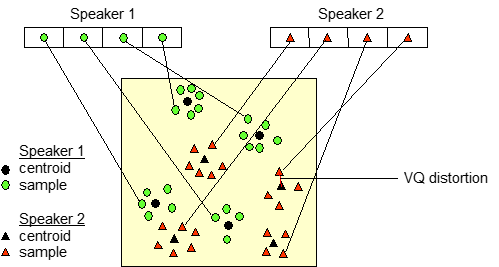
\includegraphics[width=.8\textwidth]{Picture3.png}
    \caption{Conceptual diagram illustrating vector quantization codebook formation. One speaker can be discriminated from another based of the location of centroids. (Adapted from Song et al., 1987)
    }
    \label{fig:VQ}
\end{figure}

\subsubsection{Clustering the Training Vectors}
After the enrolment session, the feature vectors extracted from input speech of each speaker provide a set of training vectors for that speaker.  As described above, the next important step is to build a speaker-specific VQ codebook for each speaker using those training vectors.  There is a well-known algorithm, namely LBG algorithm [Linde, Buzo and Gray, 1980], for clustering a set of L training vectors into a set of M codebook vectors.  The algorithm is formally implemented by the following recursive procedure:

\begin{enumerate}
    \item Design a 1-vector codebook; this is the centroid of the entire set of training vectors (hence, no iteration is required here).
    \item Double the size of the codebook by splitting each current codebook $\y_n$ according to the rule:
    \begin{gather*}
        \y_n^+ = \y_n(1+\epsilon)\\
        \y_n^- = \y_n(1-\epsilon)
    \end{gather*}
    where $n$ varies from 1 to the current size of the codebook, and $\epsilon$ is a splitting parameter (we choose $\epsilon=0.01$).
    \item Nearest-Neighbor Search: for each training vector, find the codeword in the current codebook that is closest (in terms of similarity measurement), and assign that vector to the corresponding cell (associated with the closest codeword).
    \item Centroid Update: update the codeword in each cell using the centroid of the training vectors assigned to that cell.
    \item Iteration 1: repeat steps 3 and 4 until the average distance falls below a preset threshold
    \item Iteration 2: repeat steps 2, 3 and 4 until a codebook size of $M$ is designed.

\end{enumerate}

Intuitively, the LBG algorithm designs an $M$-vector codebook in stages.  It starts first by designing a 1-vector codebook, then uses a splitting technique on the codewords to initialize the search for a 2-vector codebook, and continues the splitting process until the desired $M$-vector codebook is obtained.

Fig. \ref{fig:lbg} shows, in a flow diagram, the detailed steps of the LBG algorithm.  “Cluster vectors” is the nearest-neighbor search procedure which assigns each training vector to a cluster associated with the closest codeword.  “Find centroids” is the centroid update procedure.  “Compute distortion” sums the distances of all training vectors in the nearest-neighbor search so as to determine whether the procedure has converged.

For FFT based features, however, this VQ based approach is not applicable and finding the centroid vectors of each class, i.e. the first block in Fig. \ref{fig:lbg} is enough for training as FFT based features are vectors, rather than a set of vectors.

\tikzstyle{decs} = [diamond, draw, fill=white!80!red,
    text width=3.5em, text centered, rounded corners, minimum height=3em ,aspect=2]
    
\tikzstyle{fin} = [circle, draw, fill=white!80!green,
    text width=2em, text centered]
\begin{figure}[htb]
    \centering
    \begin{tikzpicture}[scale=1, node distance = 2cm, auto]
        \node [block] (f_cent) {Find Centroid};
        \draw (2.5, -1) node [decs]  (dec_m) {$m<M$};
        \node [block, below of = f_cent] (spl_cent) {Split Centroids};
        \node [block, below of = spl_cent] (m2m) {$m=2m$};
        \node [block, below of = m2m] (cl_vec) {Cluster Vectors};
        \node [block, below of = cl_vec] (f_cents) {Find Centroids};
        \node [block, below of = f_cents]  (compd) {Compute distortion};
        \node [decs, below of = compd]  (dec_s) {$\frac{D-D'}{D}<\epsilon$};
        \node [block, left of = dec_s, node distance = 3.4cm]  (dd) {$D'=D$};
        \node [fin, right of = dec_m, node distance=2.5cm] (stop) {Stop};
        
        \path [line] (f_cent) -- (spl_cent);
        \path [line] (spl_cent) -- (m2m);
        \path [line] (m2m) -- (cl_vec);
        \path [line] (cl_vec) -- (f_cents);
        \path [line] (f_cents) -- (compd);
        \path [line] (compd) -- (dec_s);
        \path [line] (dec_s) -- node [above, color=black] {No} (dd);
        \path [line] (dec_s) -| node [right, color=black] {Yes} (dec_m);
        \path [line] (dec_m) -- node [above, color=black] {No} (stop);
        \path [line] (dec_m) -| node [above right, color=black] {Yes} (spl_cent);
        \path [line] (dd) |- (cl_vec);
    \end{tikzpicture}
    \caption{Flow diagram of LBG algorithm.}
    \label{fig:lbg}
\end{figure}
\section{Project}
As stated before, in this project we will experiment with the building and testing of an automatic speaker recognition system. D2L Project folder provides a test database and some functions to ease the development process.  You can find two main functions: \texttt{train} and \texttt{test}. Download all of these files from the project web page into your working folder.  These files need to be thoroughly understood.  Your tasks are to write missing parts for feature extraction and matching, which will be called from the given main functions.  In order to accomplish that, follow each step in this section carefully and check your understanding by answering all the questions.

\subsection{Speech Data}
Download the ZIP file of the speech database from the project D2L page. After unzipping the file correctly, you will find two folders, TRAIN and TEST, each contains 8 files, named: S1.WAV, S2.WAV, …, S8.WAV; each is labeled after the ID of the speaker.  These files were recorded in Microsoft WAV format.  In Windows systems, you can listen to the recorded sounds by double clicking into the files.

Our goal is to train a voice model (or more specific, a VQ codebook in the MFCC vector space) for each speaker S1 - S8 using the corresponding sound file in the TRAIN folder.  After this training step, the system would have knowledge of the voice characteristic of each (known) speaker.   Next, in the testing phase, the system will be able to identify the (assumed unknown) speaker of each sound file in the TEST folder.

\textcolor{red}{\textbf{Question 1:}} \textit{Play each sound file in the }\texttt{data/train} \textit{folder.  Can you distinguish the voices of the eight speakers in the database?  Now play each sound in the} \texttt{data/test} \textit{folder in a random order without looking at the file name (pretending that you do not known the speaker) and try to identify the speaker using your knowledge of their voices that you just learned from the} \texttt{data/train} \textit{folder.  This is exactly what the computer will do in our system.  What is your (human performance) recognition rate?  Record this result so that it could be later on compared against the performance of our system.}

\subsection{Speech Processing}
In this phase you are required to write a function that reads a sound file and turns it into an array of FFT, a sequence of STFT, or a sequence of MFCC (acoustic vectors) using the speech processing steps described previously. Many of those tasks are already accomplished by standard functions in \texttt{scipy.signal} library.  The functions that you might need are: \href{https://docs.python.org/3/library/wave.html}{\texttt{wave}}\footnote{You can utilize \texttt{scipy.io.wavfile} as well.}, \href{https://docs.scipy.org/doc/scipy-0.19.1/reference/generated/scipy.signal.hamming.html}{\texttt{scipy.signal.hamming}}, \href{https://docs.scipy.org/doc/scipy/reference/generated/scipy.fft.fft.html#scipy.fft.fft}{\texttt{scipy.fft.fft}}, \href{https://docs.scipy.org/doc/scipy/reference/generated/scipy.signal.stft.html}{\texttt{scipy.signal.stft}}, \href{https://docs.scipy.org/doc/scipy/reference/generated/scipy.fft.dct.html}{\texttt{scipy.fft.dct}} and \href{https://pytorch.org/audio/main/tutorials/audio_feature_extractions_tutorial.html#mel-filter-bank}{\texttt{melfilter}}.  

\textcolor{red}{\textbf{Question 2:}} \textit{Read a sound file.  Check it by playing the sound file using \texttt{scipy.io}.  What is the sampling rate?  What is the highest frequency that the recorded sound can capture with fidelity? With that sampling rate, how many milliseconds of actual speech are contained in a block of 256 samples? Plot the signal to view it in the time domain. Convert it into frequency domain using \texttt{scipy.fft.fft} and plot the frequency information. It should be obvious that the raw signal in the time or frequency domain has a very high amount of elements and it is difficult to analyze the voice characteristic.
Now cut the speech signal (a vector) into frames with overlap (refer to the frame section in the theory part).  The result is a matrix where each column is a frame of $N$ samples from original speech signal.  Apply the steps “Windowing” and “FFT” to transform the signal into the frequency domain.}

\textcolor{red}{\textbf{Question 3:}} \textit{After successfully running the preceeding process, what is the interpretation of the result?  Compute the power spectrum and plot it out using the \texttt{plt.matshow} command.  Note that it is better to view the power spectrum on the log scale.  Locate the region in the plot that contains most of the energy.  Translate this location into the actual ranges in time (ms) and frequency (in Hz) of the input speech signal.}

\textcolor{red}{\textbf{Question 4:}} \textit{Compute and plot the power spectrum of a speech file using different frame size: for example $N = 128$, 256 and 512.  In each case, set the frame increment $M$ to be about $N/3$.  Can you describe and explain the differences among those spectra?}

The last step in speech processing is converting the power spectrum into mel-frequency cepstrum coefficients. The function \href{https://pytorch.org/audio/main/tutorials/audio_feature_extractions_tutorial.html#mel-filter-bank}{\texttt{melfilter}} can be useful for this task.

\textcolor{red}{\textbf{Question 5:}} \textit{Check the link given above for more information about this function.  Follow the tutorial to plot out the mel-spaced filter bank. What is the behavior of this filter bank?  Compare it with the theoretical part.}

\textcolor{red}{\textbf{Question 6:}} \textit{Compute and plot the spectrum of a speech file before and after the mel-frequency wrapping step.  Describe and explain the impact of the} \href{https://pytorch.org/audio/main/tutorials/audio_feature_extractions_tutorial.html#mel-filter-bank}{\texttt{melfilter}} \textit{program.}

Finally, complete the “Cepstrum” step and put all pieces together into a single function, which performs the preprocessing. For this part, it is always recommended to have a single function for preprocessing, which in turn calls other functions depending on the feature type you need to work with, such as STFT or MFCC. See \texttt{preprocess} function in the project folder for an example.

\subsection{Vector Quantization}
The result of the last section is that we transform speech signals into vectors in an acoustic space.  In this section, we will apply the VQ-based pattern recognition technique to build speaker reference models from those vectors in the training phase and then can identify any sequences of acoustic vectors uttered by unknown speakers (see the paper ‘Speaker Recognition Using MFCC and Vector Quantization’ by Nijhawan and Soni, 2014).

\textcolor{red}{\textbf{Question 7:}} \textit{To inspect the feature space (STFT or MFCC vectors) we can pick any two dimensions (say the 5th and the 6th) and plot the data points in a 2D plane.  Use acoustic vectors of two different speakers and plot data points in two different colors.  Do the data regions from the two speakers overlap each other?  Are they in clusters?}

Now write a function, \texttt{vqlbg}, that trains a VQ codebook  with 8 classes corresponding to the 8 speakers using the LGB algorithm described before.  Use the utility function \href{https://docs.scipy.org/doc/scipy/reference/generated/scipy.spatial.distance.cdist.html#scipy.spatial.distance.cdist}{\texttt{scipy.spatial.distance.cdist}} to compute the pairwise Euclidean distances between the codewords and training vectors in the iterative process.

\subsection{Simulation and Evaluation}
Now is the final part!  Use the two supplied programs: train and test to simulate the training and testing procedure in a speaker recognition system, respectively.

\textcolor{red}{\textbf{Question 8:}} \textit{What is recognition rate our system can perform?  Compare this with the human performance.  For the cases that the system makes errors, re-listen to the speech files and try to come up with some explanations.}



\end{document}